% Time-stamp: <2022-11-08 07:39:29 A13258Q>
% Amine Raboun 2023, https://amineraboun.github.io/
% Romain Lafarguette 2023, https://romainlafarguette.github.io/

%% ---------------------------------------------------------------------------
%% Preamble: Packages and Setup
%% ---------------------------------------------------------------------------
% Class 
\documentclass{beamer}

% Theme
\usetheme{Boadilla}
\usecolortheme{dolphin}
%\setbeamertemplate{headline}{} % Remove the top navigation bar

% Font and encoding
\usepackage[utf8]{inputenc} % Input font
\usepackage[T1]{fontenc} % Output font
\usepackage{lmodern} % Standard LateX font
\usefonttheme{serif} % Standard LateX font

% Maths 
\usepackage{amsfonts, amsmath, mathabx, bm, bbm} % Maths Fonts

% Graphics
\usepackage{graphicx} % Insert graphics
\usepackage{subfig} % Multiple figures in one graphic
\graphicspath{{/../static/img}{/../static/diagrams}}



% Layout
\usepackage{changepage}

% Colors
\usepackage{xcolor}
\definecolor{imfblue}{RGB}{0,76,151} % Official IMF color
\setbeamercolor{title}{fg=imfblue}
\setbeamercolor{frametitle}{fg=imfblue}
\setbeamercolor{structure}{fg=imfblue}

% Tables
\usepackage{booktabs,rotating,multirow} % Tabular rules and other macros
%\usepackage{pdflscape,afterpage} % Landscape mode and afterpage
%\usepackage{threeparttable} % Split long tables
\usepackage[font=scriptsize,labelfont=scriptsize,labelfont={color=imfblue}]{caption}

% Import files
\usepackage{import}

% Appendix slides
\usepackage{appendixnumberbeamer} % Manage page numbers for appendix slides

% References
\usepackage{hyperref}

% A few macros: environments
\newenvironment{wideitemize}{\itemize\addtolength{\itemsep}{10pt}}{\enditemize}
\newenvironment{wideenumerate}{\enumerate\addtolength{\itemsep}{10pt}}{\endenumerate}

\newenvironment{extrawideitemize}{\itemize\addtolength{\itemsep}{30pt}}{\enditemize}
\newenvironment{extrawideenumerate}{\enumerate\addtolength{\itemsep}{30pt}}{\endenumerate}

% Remove navigation symbols and other superfluous elements
\setbeamertemplate{navigation symbols}{}
\beamertemplatenavigationsymbolsempty

%\setbeamertemplate{note page}[plain]
\hypersetup{pdfpagemode=UseNone} % don't show bookmarks on initial view
\setbeameroption{hide notes}

% Institute font
\setbeamerfont{institute}{size=\footnotesize}
\DeclareMathSizes{10}{9}{7}{5}  

%% ---------------------------------------------------------------------------
%% Title info
%% ---------------------------------------------------------------------------
\title[Core Concepts]{Introduction to key Statistical Concepts}
\author[Lafarguette \& Raboun]{Romain Lafarguette, Ph.D. Amine Raboun, Ph.D.}
\institute[IMF STX]{Quant \& IMF External Expert\thanks{\scriptsize{\emph{This training material is the property of the International Monetary Fund (IMF) and is intended for use in IMF courses. Any reuse requires the permission of the IMF.}}} \\
\begin{center}
{\href{https://romainlafarguette.github.io/}{\textcolor{imfblue}{https://romainlafarguette.github.io/}}} \end{center}
\begin{center}
{\href{https://amineraboun.github.io/}{\textcolor{imfblue}{https://amineraboun.github.io/}}} \end{center}
} 

\date[STI, 17 April 2023]{Singapore Training Institute, 17 April 2023}

\titlegraphic{\vspace{-0.75cm}
    \begin{figure}
    \centering
    \subfloat{{
\includegraphics[width=2cm]{../static/img/imf_logo}}}%
    \end{figure}}


% Slide between sections
\AtBeginSection[]
{
    \begin{frame}
        \frametitle{Table of Contents}
        \tableofcontents[currentsection]
    \end{frame}
}

%% ---------------------------------------------------------------------------
%% Title slide
%% ---------------------------------------------------------------------------
\begin{document}

\begin{frame}
\maketitle
\end{frame}

\begin{frame}
  \frametitle{Resources}
  This course is based on several free and open-source references available on line
  \begin{wideitemize}
    \item Rob Hyndman handbook: \href{https://otexts.com/fpp3/}{\beamergotobutton{https://otexts.com/fpp3/}} 
    \item Christophe Hurlin's slides: \href{https://sites.google.com/view/christophe-hurlin/teaching-resources}{\beamergotobutton{https://sites.google.com/view/christophe-hurlin/teaching-resources}}
    \item At the introductory level: \emph{Basic Econometrics} (2008) by Damodar Gujarati and Dawn Porter's. They have 5 chapters on time series       
    \item A good book on time series analysis for finance: \emph{The Econometric Modelling of Financial Time Series} (2008), by Terence C. Mills and Raphael N. Markellos
    \item The main reference is Hamilton, but is difficult to read...: \emph{Time Series Analysis} (1994), by James Hamilton 
  \end{wideitemize}
\end{frame}

\begin{frame}{Outline of the Course}
\tableofcontents
\end{frame}


\section{Data Concepts}

\begin{frame}
  \frametitle{Overview}

Financial econometrics (including time-series econometrics) are based on four main elements:\\
\medskip

  \begin{wideenumerate}
    \item A sample of data
    \item An econometric model, based on a theory or not
    \item An estimation method to estimate the coefficients of the model
    \item Inference/testing approach to validate the estimation
  \end{wideenumerate}
  
\end{frame}


\begin{frame}
  \frametitle{Data Types}

  In econometrics, sets can be mainly distinguished in three types:\\
  \medskip
  
  \begin{wideenumerate}
    \item Cross-sectional data
    \item Time series data
    \item Panel data
  \end{wideenumerate}
  
\end{frame}

\begin{frame}
  \frametitle{Cross-Sectional Data}
  Cross-sectional data are the most common type of data encountered in statistics and econometrics.\\
  \medskip

  
  \begin{wideitemize}
    \item Data at the entities level: banks, countries, individuals, households, etc.
    \item \textbf{No time dimension}: only one "wave" or multiple waves of different entities
    \item Order of data does not matter: no time structure
  \end{wideitemize}
\end{frame}


\begin{frame}
  \frametitle{Time Series Data}

  Time series data are very common in financial econometrics and central banking. They entail specific estimation methods to do the \textbf{time-dependence}.\\

  \medskip
  
  \begin{wideitemize}
    \item Data for a single entity (person, bank, country, etc.) collected at multiple time periods. Repeated observations of the same variables (interest rate, GDP, prices, etc.)
    \item Order of data is important!
    \item The observations are typically not independent over time
  \end{wideitemize}  
\end{frame}


\begin{frame}
  \frametitle{Panel/Longitudinal Data}
  Panel data contain the most information and allow for more complex estimation and analysis.\\

  \medskip

  \begin{wideitemize}
    \item Data for multiple entities (individuals, firms, countries, banks, etc.) in which outcomes and characteristics of each entity are observed at multiple points in time
    \item Combine cross-sectional and time-series information
    \item Present several advantages with respect to cross-sectional and time series data, depending on the topic at hands
  \end{wideitemize}
\end{frame}

\begin{frame}
  \frametitle{Difference between Cross-Sectional and Panel Data}
  \makebox[\linewidth]{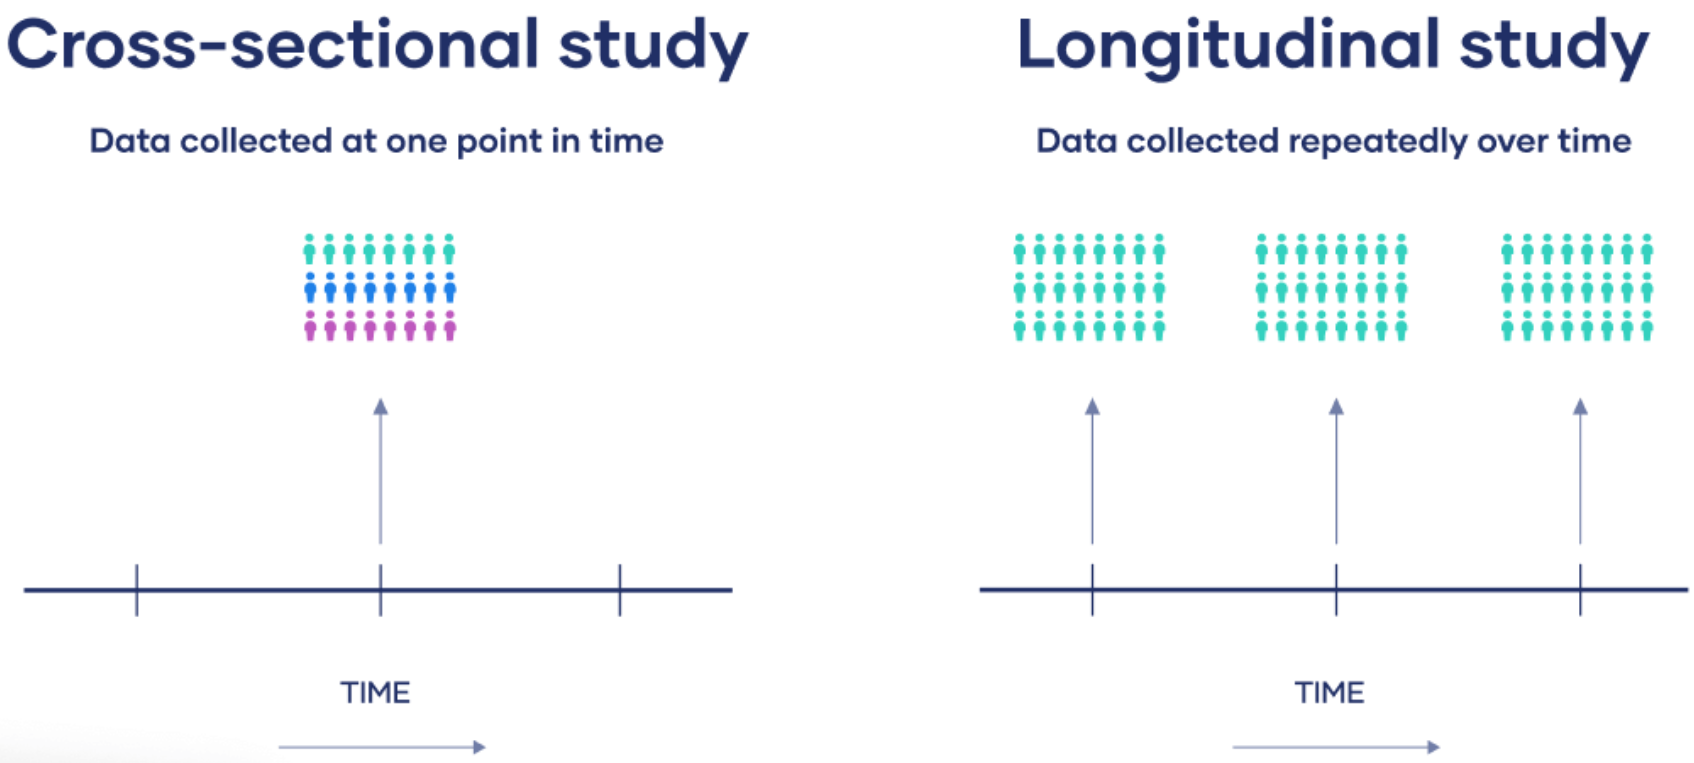
\includegraphics[width=0.8\paperwidth]{../static/course_1_img/cross_sectional_studies.PNG}}
  \hspace*{15pt}\hbox{\scriptsize Source:\thinspace{\scriptsize\itshape cdn.scribbr.com/wp-content/uploads//2020/05/x-sectional-vs-long-graphic.png}}
\end{frame}


\begin{frame}
  \frametitle{Population vs. Sample}

  \begin{block}{Definition: Population}
    A \textbf{population} is defined as including all entities (e.g. banks or firms) or all the time periods of the processus that has to be explained
  \end{block}

\smallskip
  
  \begin{wideitemize}
    \item In most cases, it is impossible to observe the entire statistical population, due to constraints (recording period, cost, etc.)
    \item A researcher would instead observe a \textbf{statistical sample} from the population. He will estimate an econometric model to understand the \textbf{properties on the population as a whole}.
  \end{wideitemize} 
\end{frame}


\begin{frame}
  \frametitle{Population vs. Sample}
  \makebox[\linewidth]{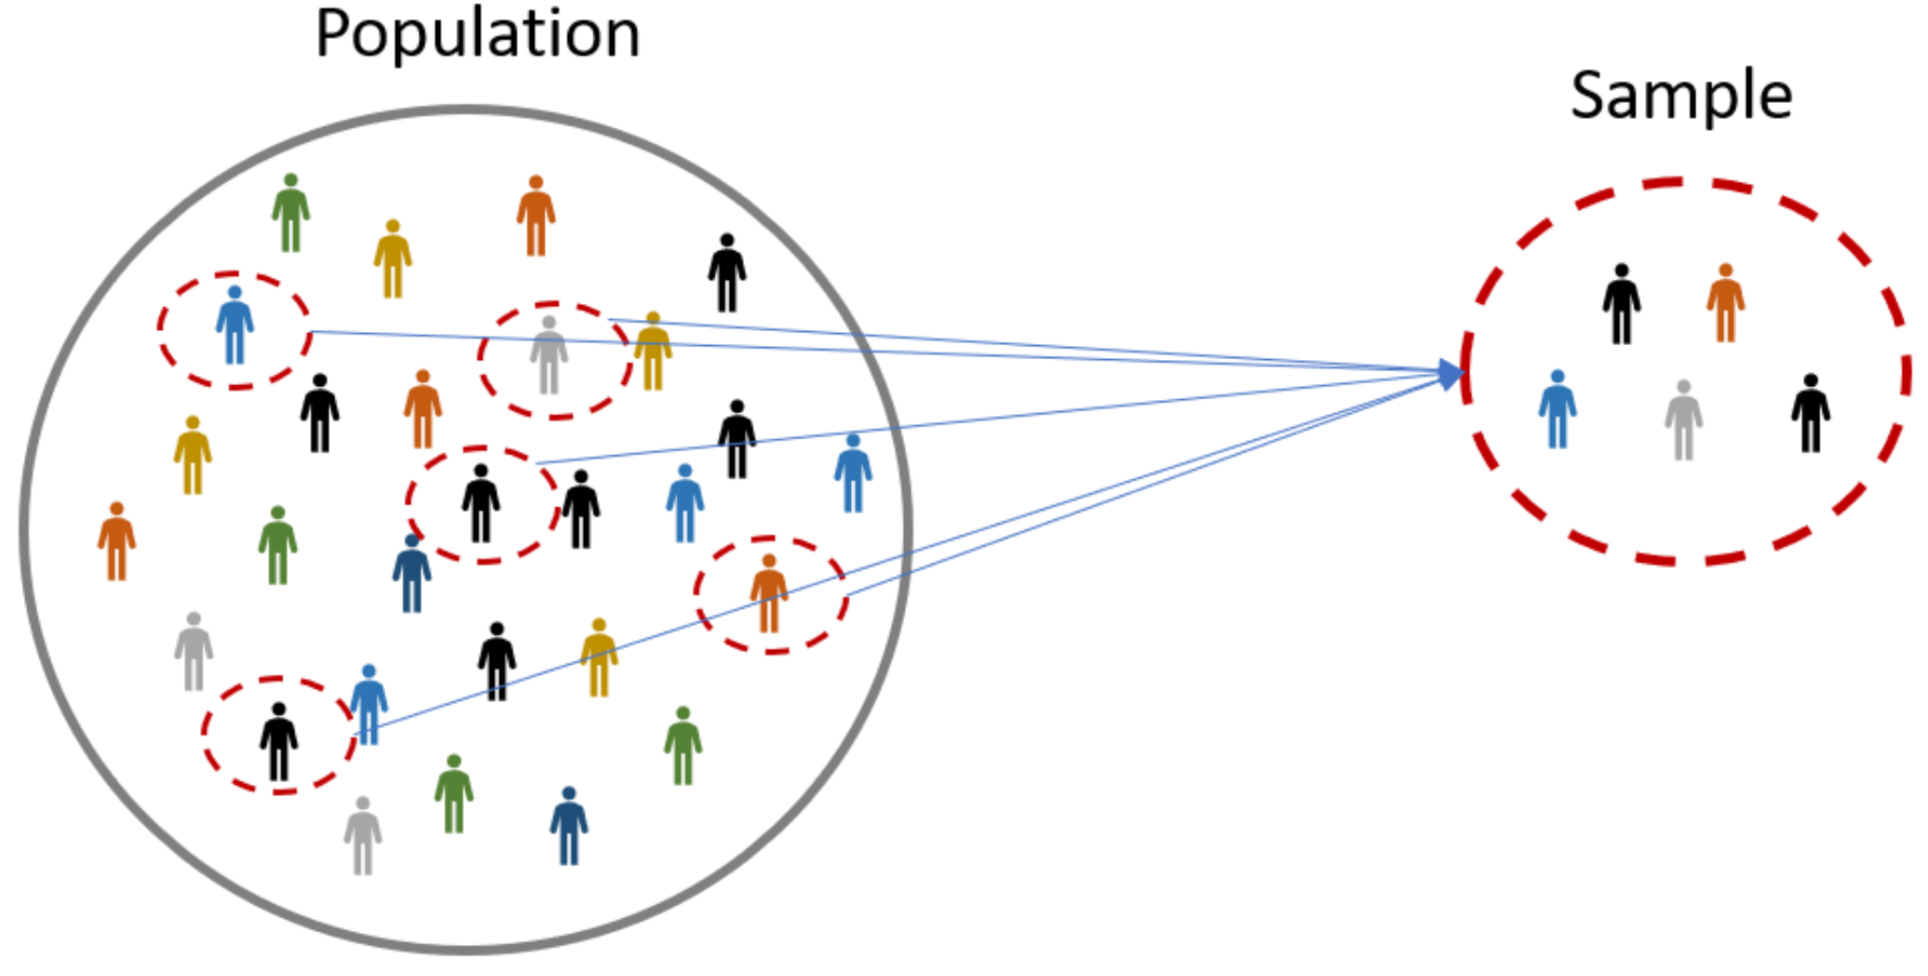
\includegraphics[width=0.8\paperwidth]{../static/course_1_img/population_sample.PNG}}
  \hspace*{15pt}\hbox{\scriptsize Credit:\thinspace{\scriptsize\itshape medium.com/analytics-vidhya}}
\end{frame}

    
\begin{frame}
  \frametitle{Data Generating Process}
  
  \begin{block}{Definition: Data Generating Process}
    \begin{itemize}
    \item A \textbf{Data Generating Process (DGP)} is a process in the real world that "generates" the data (or the sample) of interest.
    \item The process is represented by random variable (see after) $X_t$; the observation $x_t$ is one possible realization of $X_t$
    \item Given that we observe a set of $x_1, \dots, x_T$ what can we \textbf{infer} about the process $X_1, \dots, X_T$ that has generated them?
    \end{itemize}        
  \end{block}

  \begin{wideenumerate}
    \item DGP: "true" model that generated the data $x_1, \dots, x_t$
    \item But we only observe the time series a \textbf{finite number of times}
    \item However, it is convenient to allow - theoretically - the number of observations to be \textbf{infinite}: $\{X_t\}_{t \ \in \ \mathbb{Z}}$. In this case,$\{X_t\}_{t \ \in \ \mathbb{Z}}$ is called a discrete time \textbf{stochastic process} 
  \end{wideenumerate}

  
\end{frame}

\begin{frame}
  \frametitle{DGP, Population and Sample}
  \makebox[\linewidth]{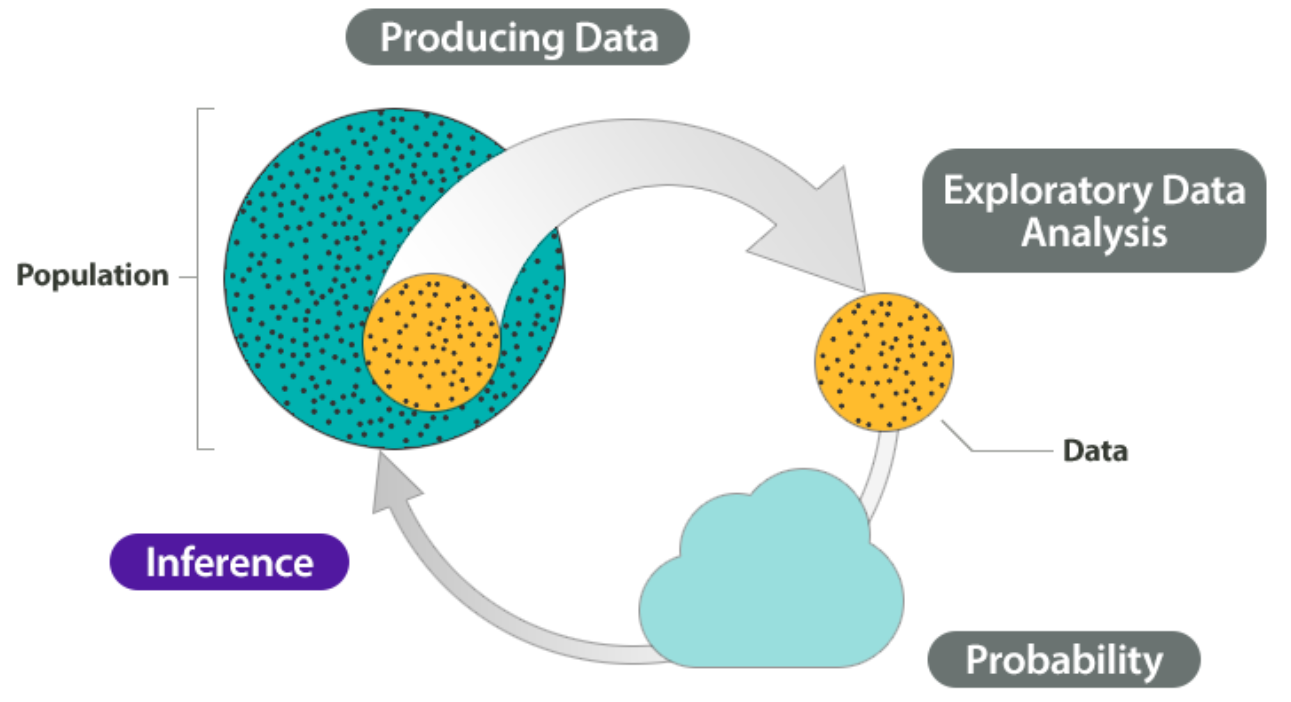
\includegraphics[width=0.8\paperwidth]{../static/course_1_img/data_generating_process.PNG}}
  \hspace*{15pt}\hbox{\scriptsize Source:\thinspace{\scriptsize\itshape bookdown.org/cristobalmoya}}
\end{frame}


\begin{frame}

  \begin{exampleblock}{Example: Data Generating Process}
    Let us assume that there is a linear relationship between interest rates in two countries ($R, R^*$), their forward ($F$) and their spot exchange rate ($S$).\\

    \begin{equation*}
      \frac{F}{S} = \frac{1+R}{1+R^*}
    \end{equation*}

    This non-arbitrage relationship (CIP) can be used in the foreign exchange market to determine the forward exchange rate

    \begin{equation*}
      \mathbb{E}[F |S=s, R=r, R^*= r^*] = s*\frac{1+r}{1+r^*}
    \end{equation*}

This relationship is the \textbf{Data Generating Process} for $F$     
  \end{exampleblock}

The equivalent of population for time series econometrics is the DGP.\\
NB: note that I use $R$ to describe the random variable and $r$ to describe its realization
  
\end{frame}


\begin{frame}
  \frametitle{Econometrics Challenge}
  The challenge of econometrics is to draw conclusions about a DGP (or population), after observing only one realization $\{x_1, \dots X_N\}$ of a random sample (the dataset). To this end, we use a statistical - or econometrics - model\\

\medskip
  
    \makebox[\linewidth]{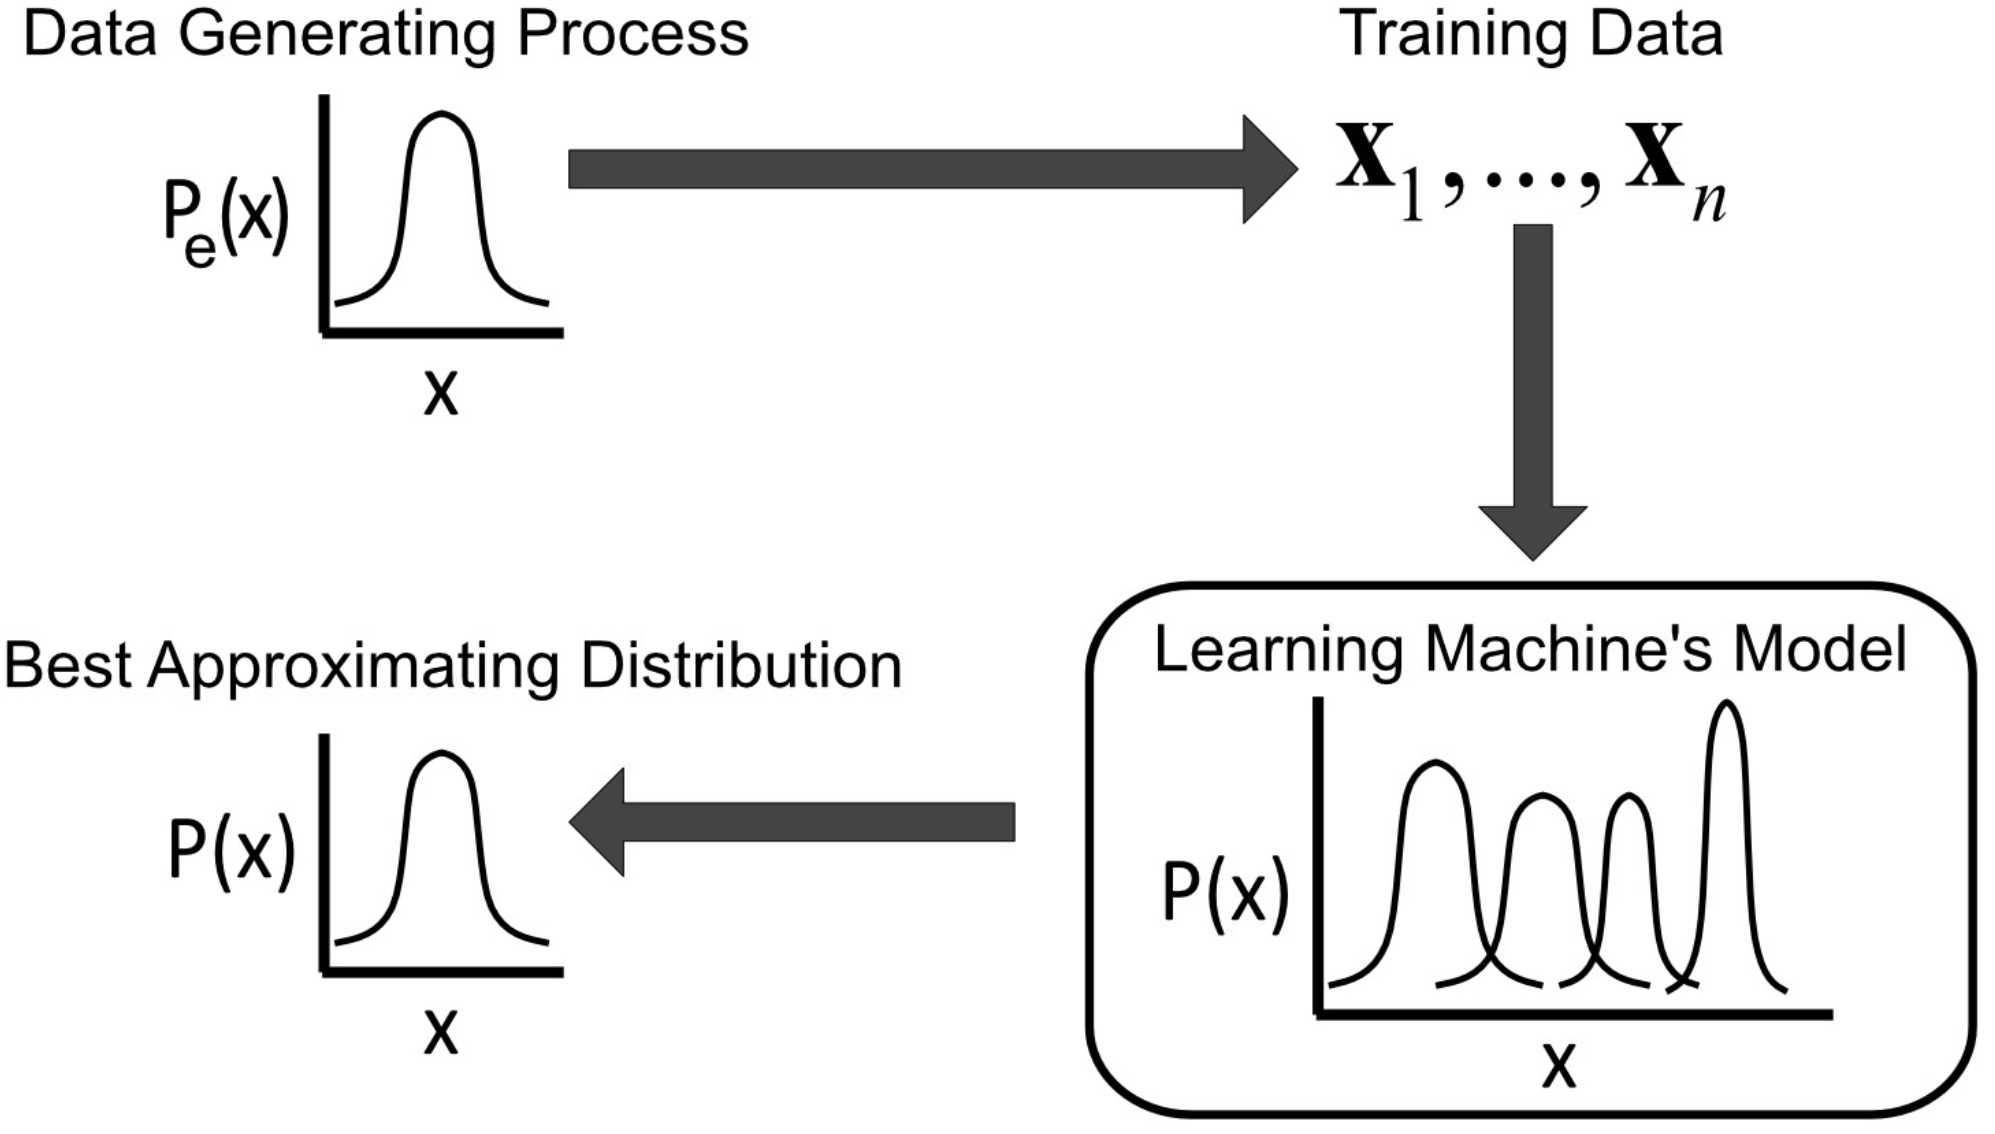
\includegraphics[height=0.6\paperheight]{../static/course_1_img/dgp_model.PNG}}
    \hspace*{15pt}\hbox{\scriptsize Source:\thinspace{\scriptsize\itshape statisticalmachinelearning.com/wp-content/uploads/2019/12/SMLframework2.jpg}}
    
\end{frame}

\section{Refresher on Probability Theory}
\begin{frame}
  \frametitle{Refresher: Random Variables}
  \begin{wideitemize}
  \item Mathematicians are formalizing and modeling randomness via the concept of \textbf{random variables}.\\
  \item Pay attention: a random variable is neither random (it is formalized via laws and distributions), not a variable (it is a function)
  \item A \textbf{random variable} is a function $f: \Omega \mapsto \mathcal{R}$ that assigns to
      a set of outcome $\Omega$ a \textbf{value}, often a real number.
  \item The probability of an outcome is equal to its \textbf{measure} divided by
        the measure of all possible outcomes
     \begin{itemize}
      \item Example: obtaining an even number by rolling a dice: $\{2, 4, 6\}$
      \item Probability to obtain an even number by rolling a dice: $m(\{2, 4,
        6\})/m(\{1, 2, 3, 4, 5, 6\}) = \frac{1}{2}$ \emph{(here, the measure
          simply "counts" the outcomes with equal weights)}
        \end{itemize}     
  \end{wideitemize}  
\end{frame}


\begin{frame}
  \frametitle{Random Variables: Intuition}
  \makebox[\linewidth]{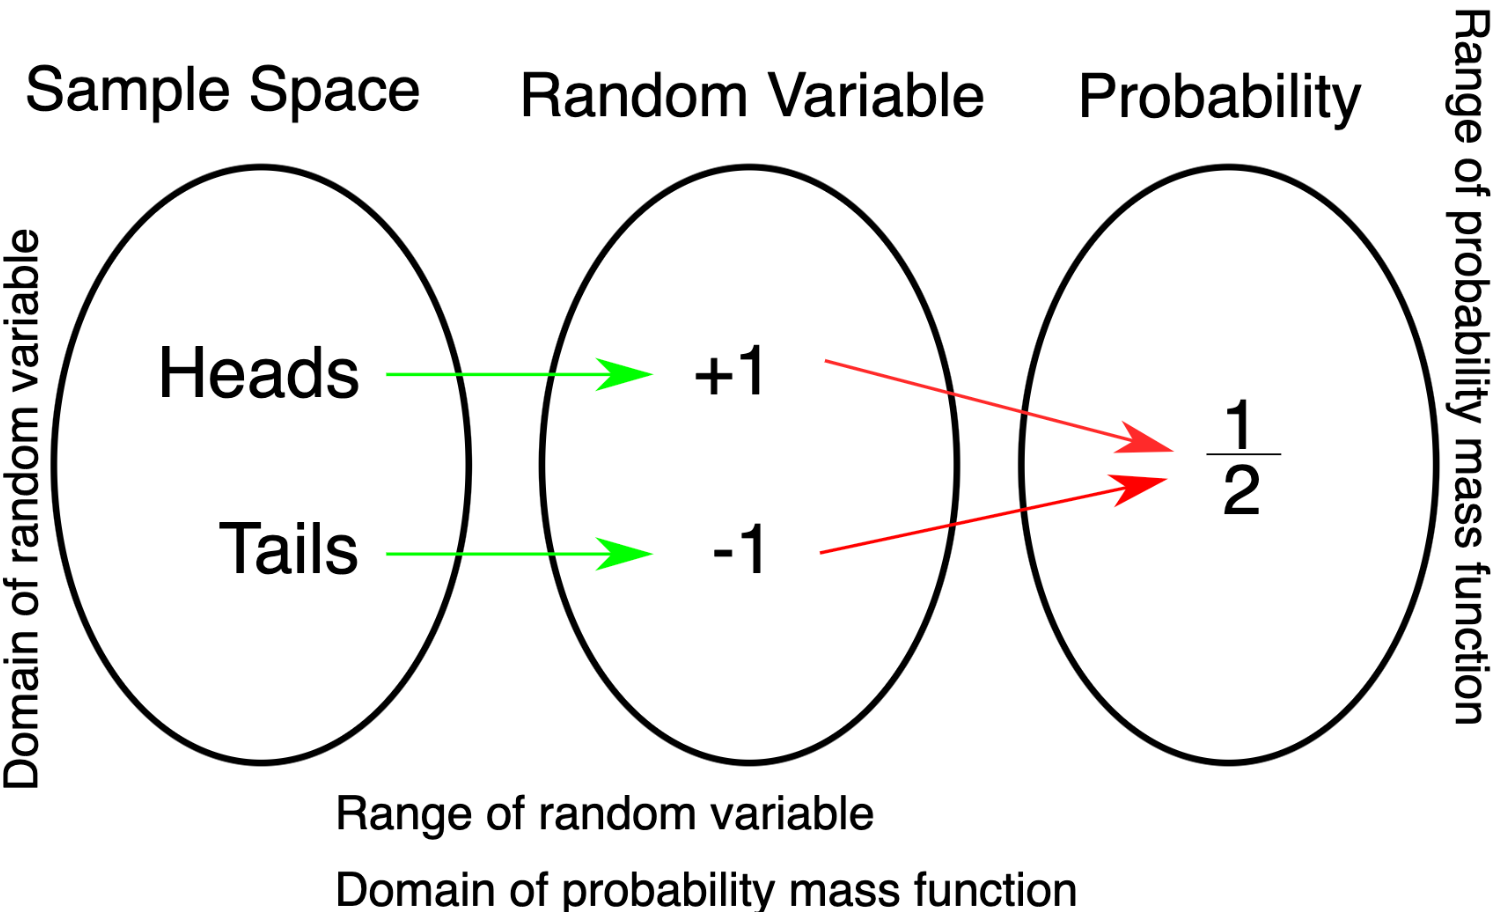
\includegraphics[width=0.8\paperwidth]{../static/course_1_img/random_variable.PNG}}
  \hspace*{15pt}\hbox{\scriptsize Source:\thinspace{\scriptsize\itshape Wikipedia}}
\end{frame}



\begin{frame}
  \frametitle{Random Variables: Mapping}
  \makebox[\linewidth]{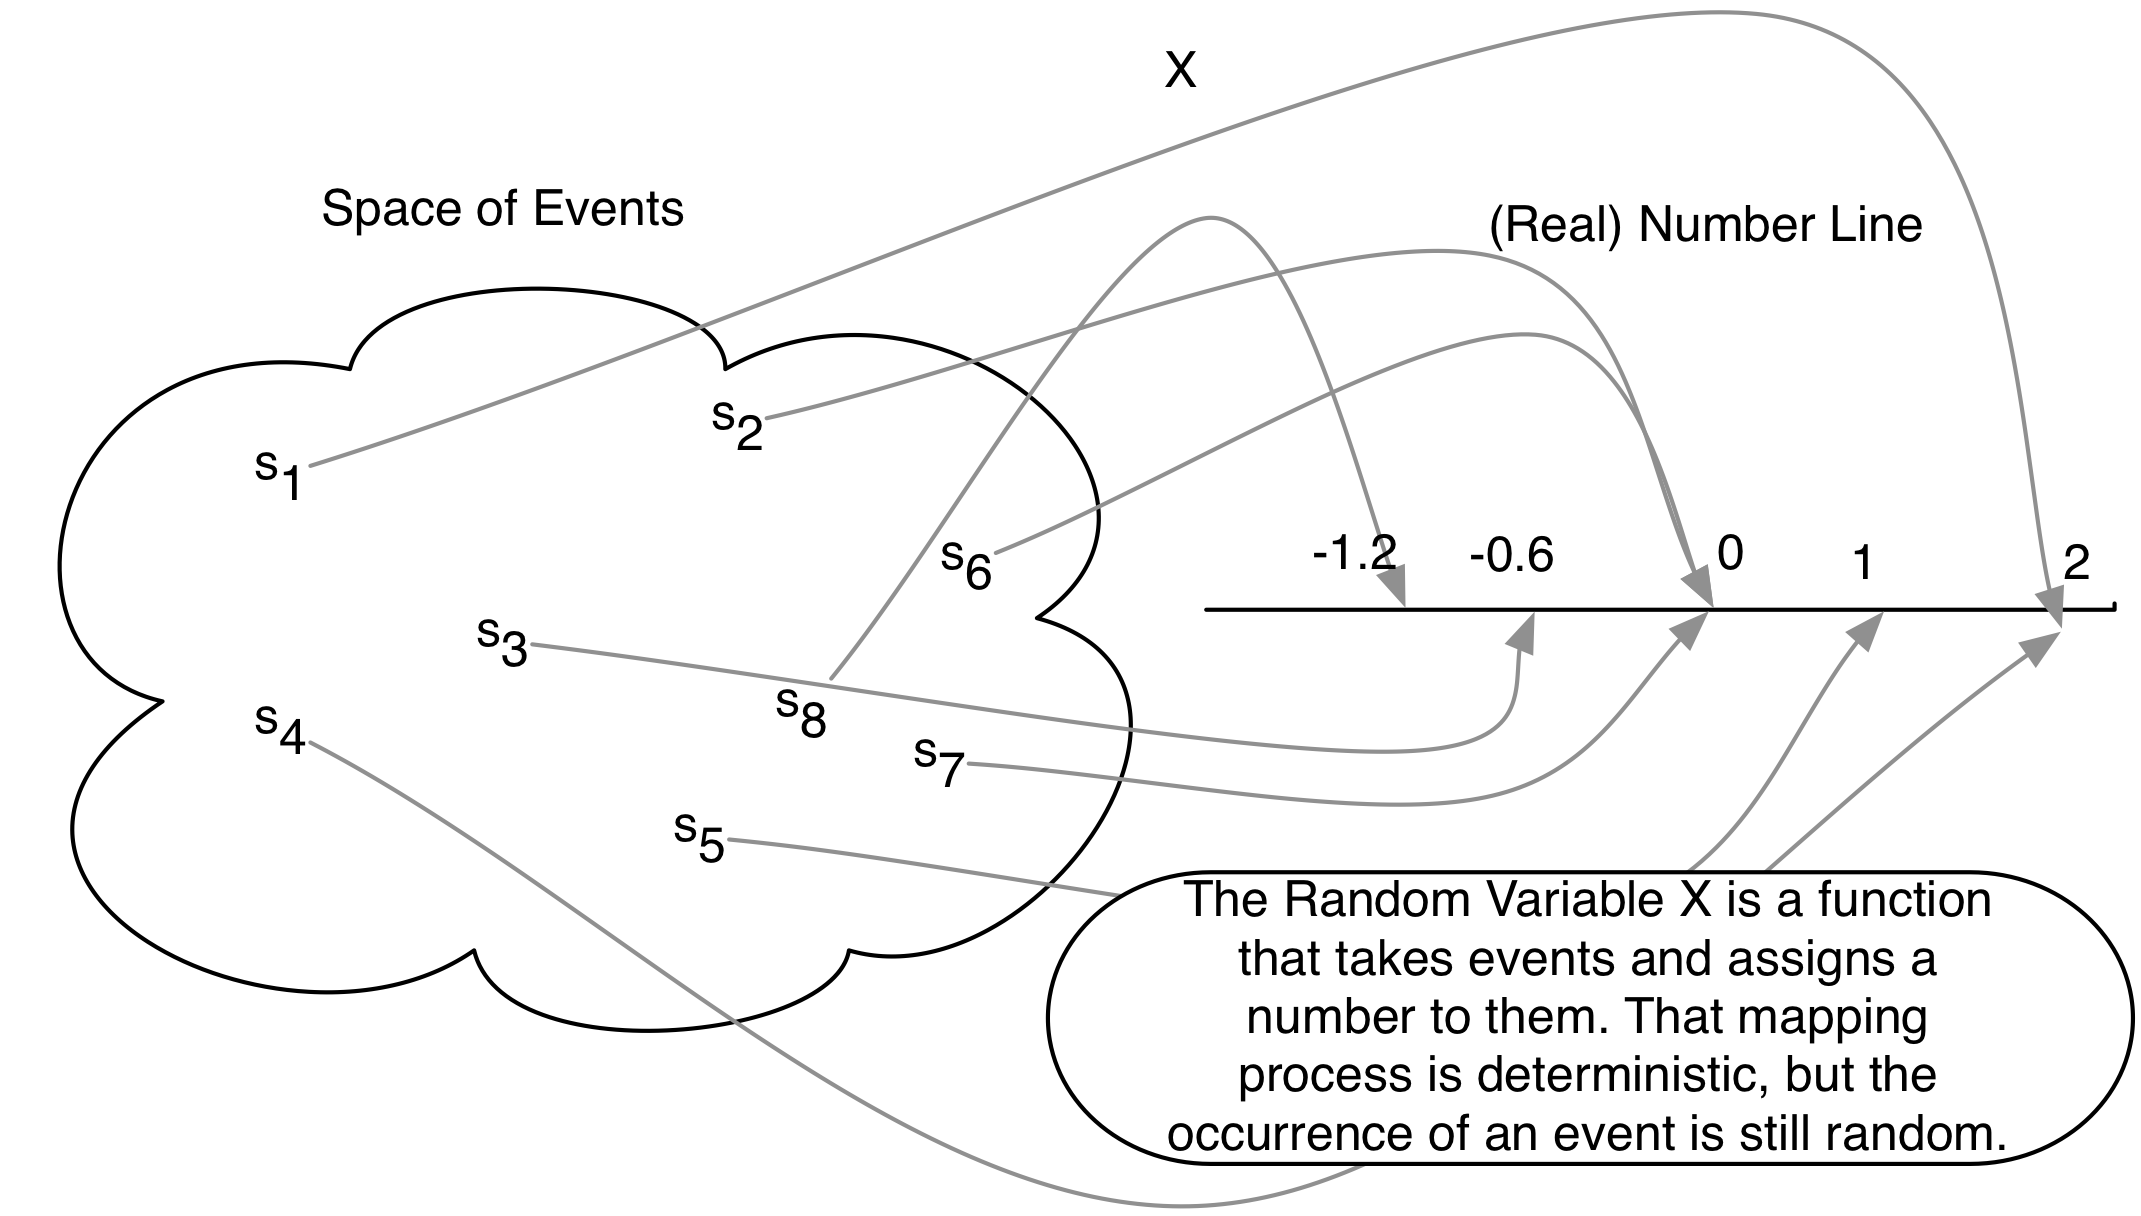
\includegraphics[width=0.8\paperwidth]{../static/course_1_img/random_variable_mapping.PNG}}
  \hspace*{15pt}\hbox{\scriptsize Credit:\thinspace{\scriptsize\itshape iqss.github.io/prefresher/images/rv.png}}
\end{frame}


\begin{frame}
  \frametitle{Random Variables (II)}    
  \begin{wideitemize}
  \item Random variables are the "building block" of statistics:
    \begin{wideitemize}
    \item Random variables are characterized by their distribution (generating
      function, moments, quantiles, etc.)
    \item The behavior of two or more random variables can be characterized by
      their dependence/independence, matrix of variance-covariance, joint
      distribution, etc.
    \item The main theorems in statistics (law of large numbers, central limit
      theorem, etc.) leverage the properties of random variables
    \end{wideitemize}
  \end{wideitemize}
\end{frame}


\begin{frame}
  \frametitle{Refresher: Probability Distributions for Continuous Variables}
  
  \begin{block}{Definition: Probability Distribution}
    The probability distribution of a random variable describes how the probabilities of the outcomes are distributed. How more likely is one outcome compared to another? Is there more upside risk or downside risk? Etc.
  \end{block}

\medskip
  
  Distributions are equivalently represented by their:
  \begin{enumerate}
  \item \textbf{The probability density function (pdf)}
  \item \textbf{The cumulative distribution function (cdf)}  
  \end{enumerate}    
  
  The pdf is also necessary to define distributions' moments (see after).\\  
\end{frame}
  
\begin{frame}{PDF and CDF}
  \begin{wideitemize}
  \item \textbf{The probability density function (pdf)} usually denoted $f_X(x0)$ (remember than $X$ stands for the random variable, while $x0$ stands for a realization of the random variable) represents the relative likelihood that the random variable $X$ will fall within a small neighborhood of $x0$ (infinitesimal concept). It is easier to conceptualize the pdf via the cdf
  \item \textbf{The cumulative distribution function (cdf)} usually denoted $F_X(x0)$ represents the probability that the random variable will be lower than $x0$. It cumulates the pdf ("all the small neighborhoods") such that:
    \begin{equation*}
F_X(x0) \equiv \mathbb{P}[X \leq x0] = \int_{-infty}^{x0} f_X(h) dh      
    \end{equation*}    
  \end{wideitemize}  
\end{frame}


\begin{frame}
\frametitle{Link between PDF and CDF}
    \makebox[\linewidth]{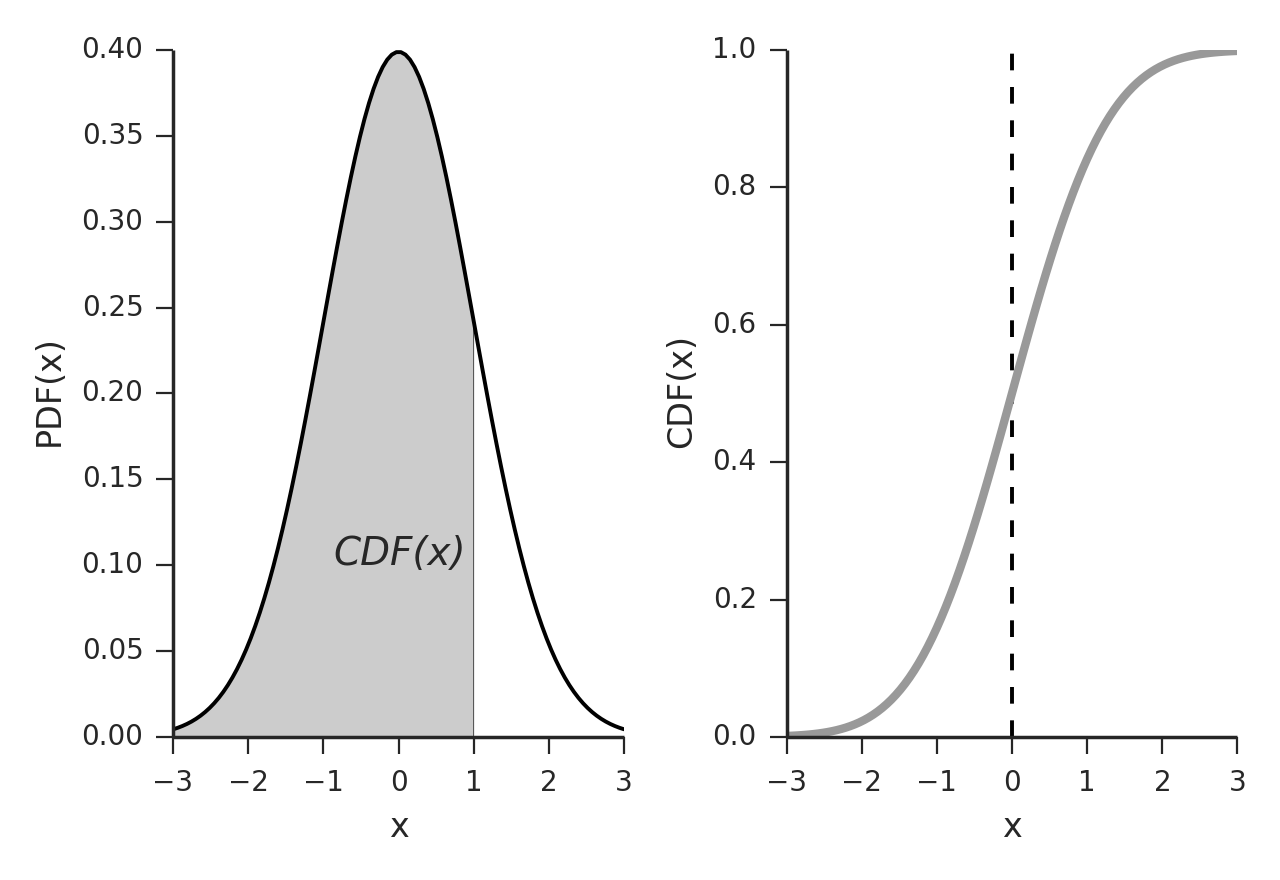
\includegraphics[width=0.85\paperwidth]{../static/course_1_img/pdf and cdf.png}}
\end{frame}


\begin{frame}
  \frametitle{Moments: Overview}
  \begin{table}
    \centering
    \begin{tabular}{lll}
      \hline
      \hline
      & Formula & Interpretation \\
      \hline
      \textbf{Mean} & $\mathbb{E}[X_t] = \mu$ & Central tendency\\
      \textbf{Variance} & $\mathbb{V}[X] = \mathbb{E}\left[(X_t - \mu)^2\right] = \sigma^2$ & Dispersion around $\mu$\\
      \textbf{Skewness} & $\mathbb{S}[X] = \mathbb{E}\left[(X_t - \mu)^3\right] = \text{sk}$ & Symmetry\\
      \textbf{Kurtosis} & $\mathbb{K}[X] = \mathbb{E}\left[(X_t - \mu)^4\right] = \kappa$ & Tail heaviness\\
      \hline
      \hline                                                                                            
    \end{tabular}
  \end{table}
\end{frame}


\begin{frame}
  \frametitle{Mean, Variance, Kurtosis}
  \makebox[\linewidth]{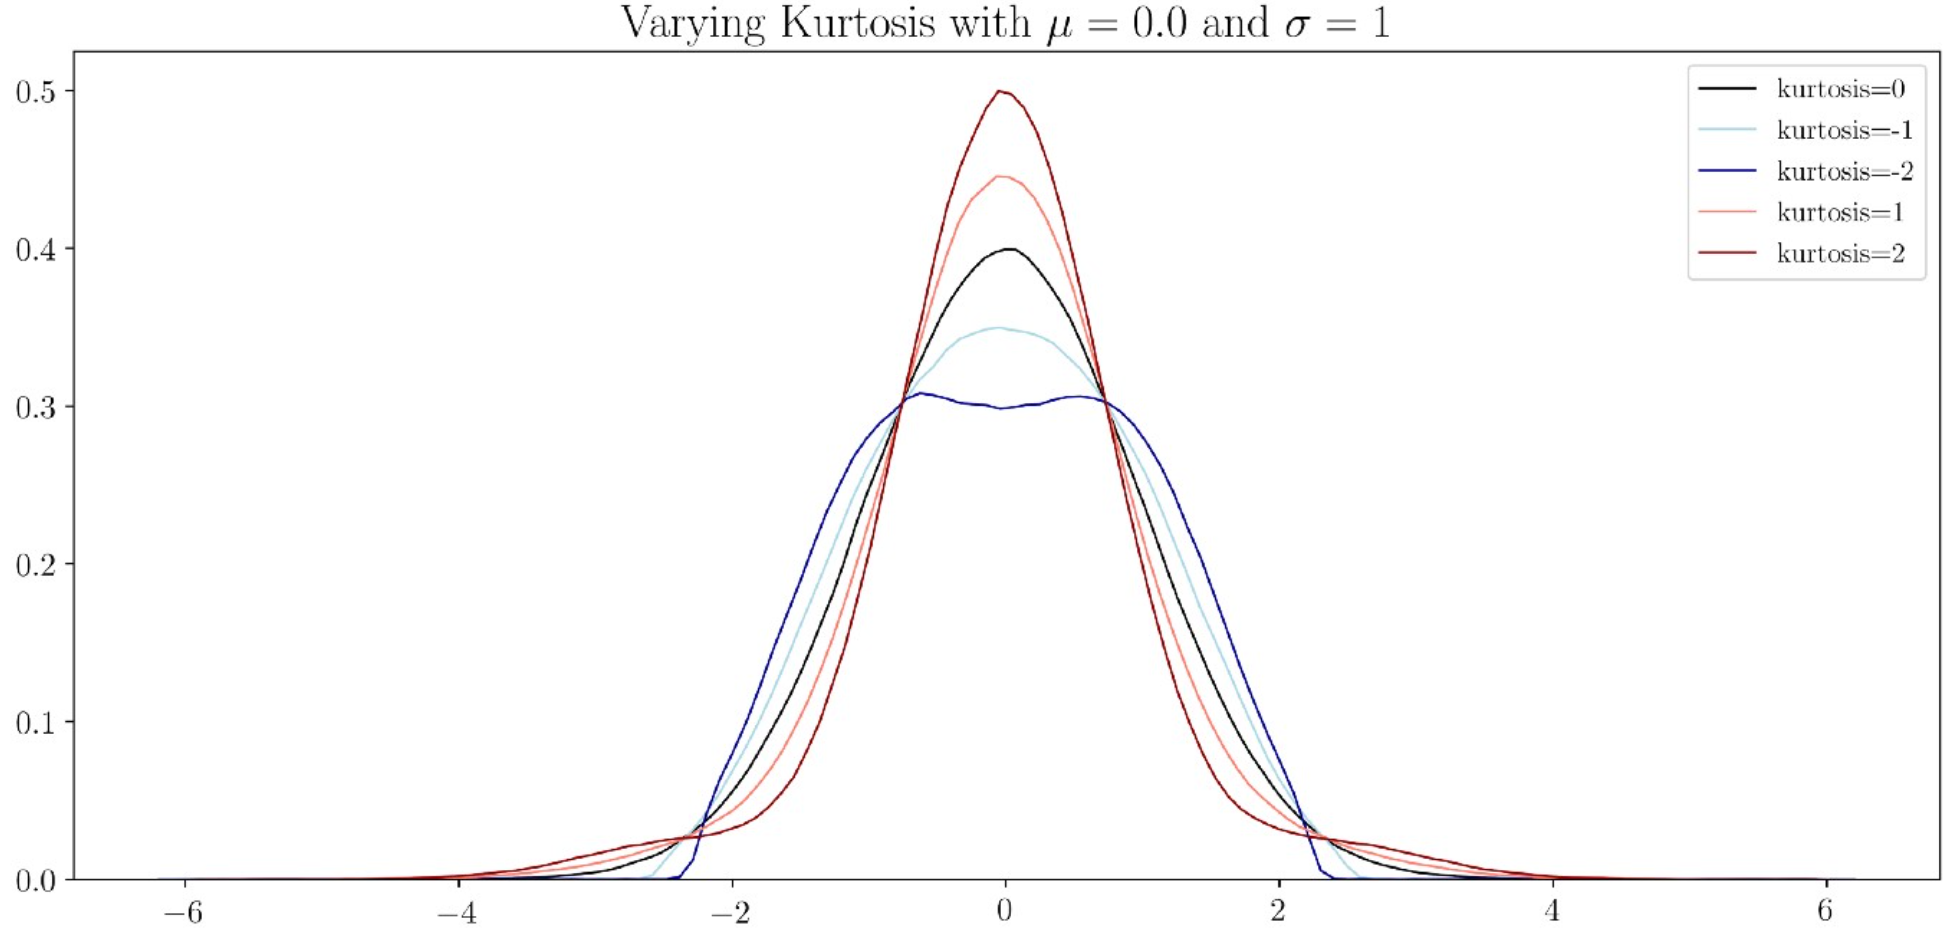
\includegraphics[width=0.8\paperwidth]{../static/course_1_img/moments_example.PNG}}
  \hspace*{15pt}\hbox{\scriptsize Credit:\thinspace{\scriptsize\itshape iqss.github.io/prefresher/images/rv.png}}
\end{frame}

\begin{frame}
  \frametitle{Kurtosis: Benchmarking against the Normal Distribution}
  There are different shapes of kurtosis 

 \makebox[\linewidth]{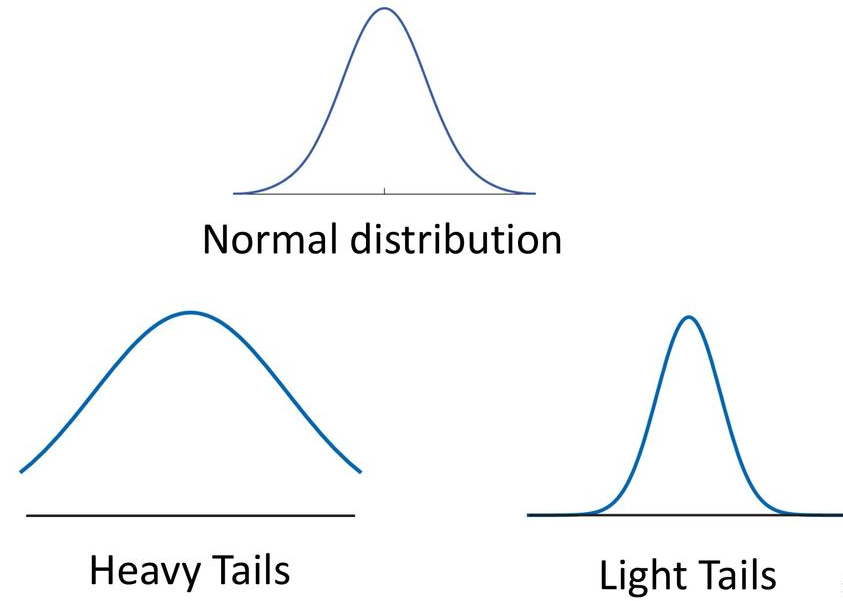
\includegraphics[width=0.7\paperwidth]{../static/course_1_img/normal versus tails.PNG}}  
\end{frame}

\begin{frame}
  \frametitle{Skewness}
  \makebox[\linewidth]{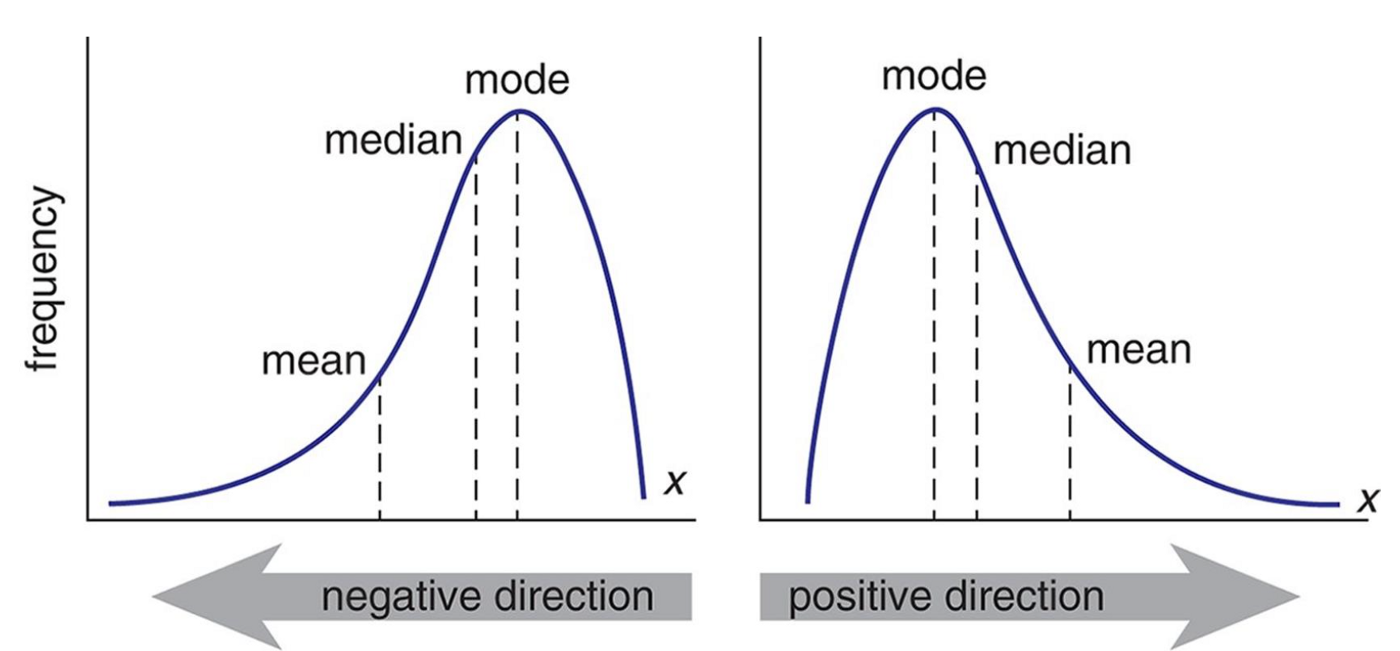
\includegraphics[width=0.8\paperwidth]{../static/course_1_img/skewness.PNG}}
  \hspace*{15pt}\hbox{\scriptsize Credit:\thinspace{\scriptsize\itshape iqss.github.io/prefresher/images/rv.png}}
\end{frame}


\begin{frame}
  \frametitle{Moments: In Practice}

  \begin{wideitemize}
    \item The moments allow to characterize the shape of the returns distribution
    \item However, the theoretical moments are \textbf{unobservable} and need to be estimated
    \item Assume that we have a sample $\{x_1, \dots, x_T\}$ realizations of the sequence of $X_t$
  \end{wideitemize}
  
\end{frame}

\section{Statistical Inference}
\begin{frame}
  \frametitle{Estimator}

  \begin{block}{Definition: Estimator}
    An \textbf{estimator} is any function $F(x1, \dots, x_t)$ of a sample. Note that any descriptive statistics is an estimator (a simple one) 
  \end{block}


  \begin{exampleblock}{Example: Sample Mean}
    The sample mean (or overage) of a sample is an estimator of the (theoretical) mean $ \mathbb{E}[X_t] = \mu$.\\
    The estimator is simply: $\hat{\mu_t} \equiv \bar{X_t} = \frac{1}{T} \sum_{t=1}^{T}x_t$
  \end{exampleblock}
  
\end{frame}


\begin{frame}
  \frametitle{Example: Variance}

  \begin{exampleblock}{Example: Sample Mean}
    Assume that the observations are drawn from \emph{i.i.d} random variables.\\
    The \textbf{sample variance} $\hat{\sigma}^2_T = \frac{1}{T-1} \sum_{t=1}^T (x_t - \bar{x}_t)^2$
  \end{exampleblock}

\textbf{Note:} the denominator is equal to \emph{T-1} as to define a sample variance corrected for the small sample bias. 
  
\end{frame}



\begin{frame}
  \frametitle{Sampling Distribution}

  \begin{block}{Fact}
    An estimator $\hat{\theta}$ is a \textbf{random variable}
  \end{block}
  Therefore, $\hat{\theta}$ has a (marginal or conditional) \textbf{probability distribution}. This sampling distribution is characterized by a probability distribution function (pdf) $f_{\hat{\theta}}(u)$

  \begin{block}{Definition: Sampling Distributions}
    The probability distribution of an estimator is called the \textbf{sampling distribution}
  \end{block}
  The sampling distribution is described by its moments, such as expectations, variance, skewness, etc.
  \end{frame}


  \begin{frame}
    \frametitle{Point Estimate}
    \begin{block}{Definition: Estimate}
      An estimate is the realized value of an estimator (e.g. a number, in a case of a point estimate) that is obtained for a particular value $x0$. Often noted as $\hat{\theta}(x0)$ for the estimator $\hat{\theta}$
    \end{block}

    \begin{exampleblock}{Estimate of a linear regression}
      \begin{itemize}
      \item DGP $Y = \alpha + \beta*X + \epsilon$, with joint sample ${y1, \dots, y_T}, {x1, \dots, x_T}$.\\
      \item We have an estimator (for instance an OLS) of $\hat{\alpha}, \hat{\beta}$
      \item Then, for any value of $X=x_0$, we can simply project the \textbf{conditional expected estimate} $y_0 = \hat{\alpha} + \hat{\beta}*x_o + \hat{\epsilon}$
      \item If the estimator is unbiased, the fitted residuals $\hat{\epsilon} = y_t - \hat{\alpha} - \hat{\beta}*x_t$ are centered on \textbf{average}:$\mathbb{E}\left[\hat{\epsilon}\right]=0$. This is why the residual disappear from the estimate of the conditional expected estimate in an OLS... but no bias doesn't mean no variance !
      \item $\epsilon$ \& $\hat{\epsilon}$ are random variables: they determine $\hat{\alpha}, \hat{\beta}$ distributions
      \end{itemize}
    \end{exampleblock}    
  \end{frame}

\end{document}